\section{Analysis: Why the optimal vocabulary size is bounded by compute}

% Here we present analyses to explain why the optimal vocabulary size is constrained by the compute.

\begin{figure}[t]
\centering
\begin{subfigure}[b]{0.32\textwidth} 
    \centering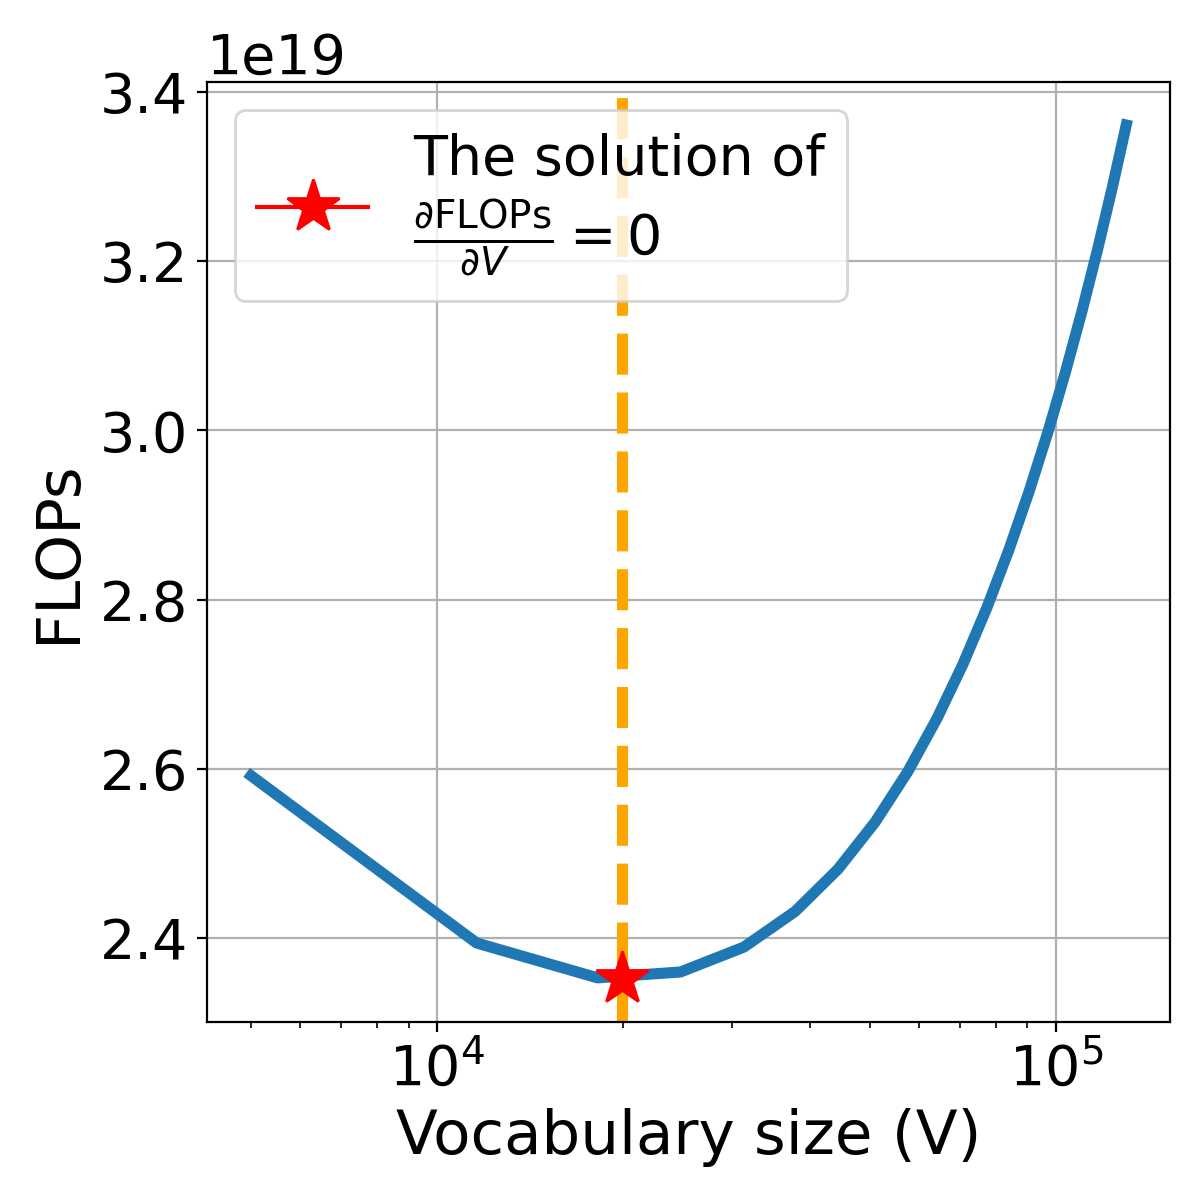
\includegraphics[width=\textwidth]{figures/derivative-flops.png}
    \label{subfig:motivation1-flops}
\end{subfigure}
\hspace{0.05\textwidth}
\begin{subfigure}[b]{0.38\textwidth} 
    \centering
    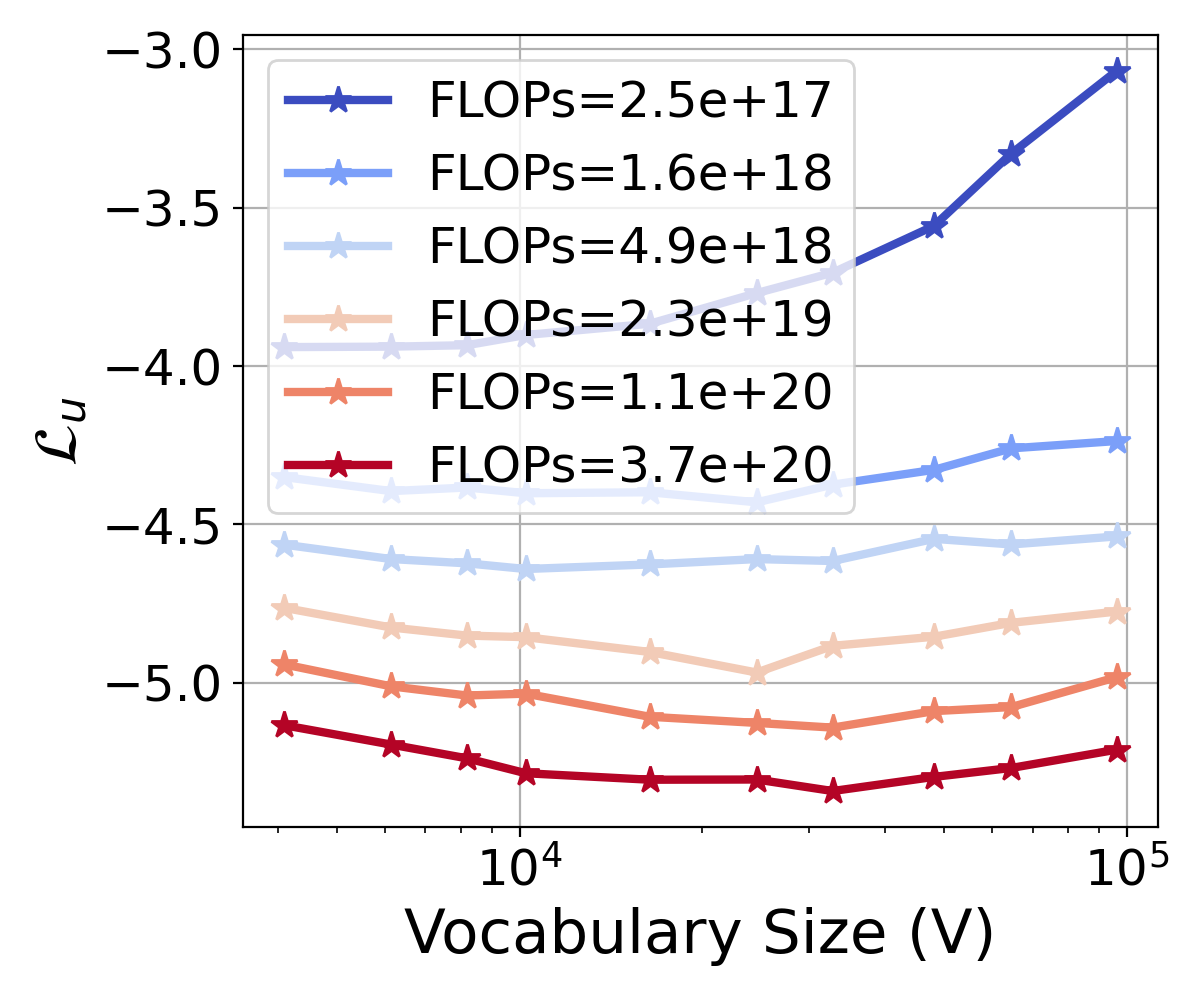
\includegraphics[width=\textwidth]{figures/motivation-ISOFlops-V-loss.png}
    \label{subfig:motivation2-flops}
\end{subfigure}    
\caption{\textbf{Left:} FLOPs curve with various vocabulary sizes, assuming all configurations achieve a fixed loss. There exists an optimal vocabulary size that minimizes FLOPs. \textbf{Right:} Loss curves with various vocabulary sizes given different FLOP budgets. For each budget there exists an optimal vocabulary size that minimizes loss. As the FLOP budget increases this optimal vocabulary size increases (shifts to the right).}
\label{fig:motivation}
\end{figure}

\textbf{Analysis 1: The perspective of fixed normalized loss}\;\;\;\;
According to~\citet{kaplan2020scaling}, the FLOPs ($C$) of a Transformer model can be estimated as $C\approx6ND$, which can be re-written as:
\begin{equation}
\label{eq:formula_C}
    C \approx 6ND \approx 6(N_{\rm nv}+Vd)Hf(V),
\end{equation}
where $N = N_{\rm nv} + N_{\rm v}$ and $D = Hf(V)$ based on \autoref{sec:preliminaries}. The reasons why model performance first increases and then decreases as the vocabulary size grows are:
(1) At small $V$, increasing the vocabulary size easily improves tokenization fertility from $f(V)$. Subsequently, more characters can be learned from the model with a fixed number of tokens, thereby improving model performance. (2) At very large $V$, the gain from tokenization fertility decreases, while the parameters from expanding the vocabulary cannot be adequately trained with limited data, which leads to a decline in model performance. We present an expanded derivation in~\autoref{append:df_dv}, and show how the corresponding FLOPs change with the vocabulary size in~\autoref{fig:motivation} (left).

\textbf{Analysis 2: The perspective of fixed FLOP budget}\;\;\;\;
Given a fixed FLOPs budget, we isolate the FLOPs and investigate how the vocabulary influences the loss. For ease, we train models with fixed $N_{nv}$ and different vocabulary sizes for the same steps, and then we use interpolation to predict the loss when FLOPs reaches the budget given the observed FLOPs and loss points. For each budget, we adopt a group of models with similar total parameters and vary vocabulary sizes. In \autoref{fig:motivation} (right) we plot the relationship between the loss w.r.t. the vocabulary size. It reveals that the vocabulary corresponding to the lowest point on the loss curve increases as the FLOPs budget increases. This suggests that with more computational resources, LLMs can harness larger vocabularies to reduce loss. However, merely expanding the vocabulary does not always lower the loss. For a fixed FLOPs budget, the loss initially decreases with the increase in vocabulary and then starts to rise, indicating that an optimal point exists for the vocabulary.
